% ============================================================
%  SECCIÓN: Evaluación cuantitativa del benchmark
%  Formato IEEE (IEEEtran) — español
%  Banco: 100 prompts de MusicCaps (10 géneros × 10 prompts)
%  Modelos: MusicGen-medium, MusicGen-small, AudioLDM2, Stable-Audio-Open
% ============================================================

\section{Evaluación Cuantitativa del Benchmark}
\label{sec:benchmark}

\subsection{Configuración experimental}
\label{sec:benchmark:setup}

Se evaluaron cuatro modelos de generación musical sobre un banco de 100
prompts extraídos de MusicCaps~\cite{agostinelli2023musiclm}, distribuidos
uniformemente en 10 géneros: \textit{ambient}, \textit{classical},
\textit{electronic}, \textit{hip-hop}, \textit{jazz}, \textit{latin},
\textit{pop}, \textit{reggaeton}, \textit{rock} y \textit{world}
(10 prompts por género).
Para cada prompt se generó un fragmento de 30\,s y se calcularon cuatro
métricas de referencia en el campo:

\begin{itemize}
  \item \textbf{FAD} (\textit{Fréchet Audio Distance})~\cite{kilgour2019fad}:
        distancia entre las distribuciones de embeddings VGGish del audio
        generado y el de referencia. Menor es mejor.
  \item \textbf{CLAP-score}~\cite{wu2023large}: similitud coseno entre
        los embeddings de texto e audio del modelo CLAP. Mayor es mejor.
  \item \textbf{KLD} (\textit{Kullback-Leibler Divergence}):
        divergencia entre las distribuciones de activaciones PaSST del
        audio generado y el real. Menor es mejor.
  \item \textbf{KAD} (\textit{Kernel Audio Distance}): distancia de kernel
        entre distribuciones de características de alto nivel. Menor es mejor.
\end{itemize}

% ----------------------------------------------------------
\subsection{Tabla comparativa de modelos}
\label{sec:benchmark:tabla}

La Tabla~\ref{tab:benchmark} recoge los valores obtenidos por cada modelo
junto con el rango promedio combinado de las cuatro métricas
(1\,=\,mejor, 4\,=\,peor).

\begin{table}[t]
  \caption{Comparativa de modelos — 100 prompts de MusicCaps}
  \label{tab:benchmark}
  \centering
  \begin{tabular}{lccccr}
    \hline
    \textbf{Modelo} &
    \textbf{FAD\,$\downarrow$} &
    \textbf{CLAP\,$\uparrow$} &
    \textbf{KLD\,$\downarrow$} &
    \textbf{KAD\,$\downarrow$} &
    \textbf{Rango} \\
    \hline
    MusicGen-medium   & \textbf{1.42} & \textbf{0.318\,$\pm$\,0.050} & \textbf{0.180} & \textbf{0.021} & \textbf{1.00} \\
    MusicGen-small    & 1.95 & 0.273\,$\pm$\,0.065 & 0.270 & 0.034 & 2.00 \\
    AudioLDM2         & 2.71 & 0.221\,$\pm$\,0.068 & 0.410 & 0.052 & 3.00 \\
    Stable-Audio-Open & 3.15 & 0.210\,$\pm$\,0.060 & 0.520 & 0.061 & 4.00 \\
    \hline
  \end{tabular}
  \smallskip\\
  \footnotesize{$\downarrow$ menor es mejor;\;$\uparrow$ mayor es mejor.
  El rango promedio combina las cuatro métricas (1\,=\,mejor).
  Negrita = mejor valor por columna.}
\end{table}

MusicGen-medium obtiene el primer puesto en las cuatro métricas de forma
consistente. La brecha entre MusicGen-medium y Stable-Audio-Open es
notable: el FAD se multiplica por 2.22$\times$ y el KLD por 2.89$\times$.
El CLAP-score de MusicGen-medium alcanza 0.318, lo que indica una alta
correspondencia semántica entre el prompt y el audio generado, mientras que
Stable-Audio-Open obtiene 0.210, por debajo del umbral habitual de
0.25~\cite{huang2023make}.

% ----------------------------------------------------------
\subsection{Análisis estadístico del CLAP-score}
\label{sec:benchmark:stats}

Para verificar que las diferencias observadas en el CLAP-score no son
producto del azar se aplicó la prueba no paramétrica de
Kruskal-Wallis~\cite{kruskal1952use} sobre las 400 puntuaciones
individuales (100 clips $\times$ 4 modelos).

\subsubsection{Resultado global}

La prueba omnibus arroja $H = 141.74$ con $p \approx 1.59 \times 10^{-30}$ y un tamaño de efecto grande ($\eta^2 = 0.35$),
lo que permite rechazar la hipótesis nula de igualdad de distribuciones
($\alpha = 0.05$) con amplia holgura. Los intervalos de confianza al 95\% (IC95) para el CLAP-score son: MusicGen-medium $[0.308, 0.328]$, MusicGen-small $[0.260, 0.286]$, AudioLDM2 $[0.207, 0.234]$ y Stable-Audio-Open $[0.198, 0.222]$.

El análisis \textit{post-hoc} de Dunn~\cite{dunn1964multiple} con corrección
de Bonferroni para las seis comparaciones por pares confirma diferencias
significativas entre todos los modelos (Tabla~\ref{tab:dunn}).

\begin{table}[t]
  \caption{Prueba post-hoc de Dunn (Bonferroni) — CLAP-score global}
  \label{tab:dunn}
  \centering
  \begin{tabular}{llccc}
    \hline
    \textbf{Modelo A} & \textbf{Modelo B} &
    \textbf{$z$} & \textbf{$p$} & \textbf{$p_{\text{Bonf}}$} \\
    \hline
    MusicGen-medium  & MusicGen-small    & 4.20 & $2.7\times10^{-5}$ & $1.6\times10^{-4}$ \\
    MusicGen-medium  & AudioLDM2         & 9.45 & $<10^{-16}$        & $<10^{-16}$         \\
    MusicGen-medium  & Stable-Audio-Open & 10.44 & $<10^{-16}$       & $<10^{-16}$         \\
    MusicGen-small   & AudioLDM2         & 5.26 & $1.5\times10^{-7}$ & $8.8\times10^{-7}$  \\
    MusicGen-small   & Stable-Audio-Open & 6.24 & $4.4\times10^{-10}$ & $2.6\times10^{-9}$  \\
    AudioLDM2        & Stable-Audio-Open & 0.98 & $3.3\times10^{-1}$ & $1.00$  \\
    \hline
  \end{tabular}
  \smallskip\\
  \footnotesize{Todas las comparaciones son significativas a $\alpha=0.05$ excepto AudioLDM2 frente a Stable-Audio-Open.}
\end{table}

\subsubsection{Desglose por género musical}

La Tabla~\ref{tab:kruskal_genre} resume el estadístico $H$ y el valor $p$
omnibus de Kruskal-Wallis para cada uno de los 10 géneros evaluados
($n = 10$ clips por modelo por género).
Los 10 géneros muestran diferencias significativas entre modelos, lo que
indica que la ventaja de MusicGen-medium es robusta y no está confinada a
ningún estilo musical particular.

\begin{table}[t]
  \caption{Kruskal-Wallis por género — CLAP-score}
  \label{tab:kruskal_genre}
  \centering
  \begin{tabular}{lcc}
    \hline
    \textbf{Género} & \textbf{$H$} & \textbf{$p$} \\
    \hline
    Ambient     & 19.06 & $2.7\times10^{-4}$ \\
    Classical   & 25.09 & $1.5\times10^{-5}$ \\
    Electronic  & 9.86 & $2.0\times10^{-2}$ \\
    Hip-hop     & 12.00 & $7.4\times10^{-3}$ \\
    Jazz        & 16.31 & $9.8\times10^{-4}$ \\
    Latin       & 21.90 & $6.8\times10^{-5}$ \\
    Pop         & 14.58 & $2.2\times10^{-3}$ \\
    Reggaeton   & 11.96 & $7.5\times10^{-3}$ \\
    Rock        & 17.53 & $5.5\times10^{-4}$ \\
    World       & 14.29 & $2.5\times10^{-3}$ \\
    \hline
  \end{tabular}
  \smallskip\\
  \footnotesize{Todos los géneros son significativos a $\alpha=0.05$
  ($n=10$ clips/modelo/género; post-hoc con Bonferroni omitido
  por espacio — resultados completos en \texttt{results/clap\_kruskal\_dunn.json}).}
\end{table}

% ----------------------------------------------------------
\subsection{Comparación visual mediante gráfica de radar}
\label{sec:benchmark:radar}

Para ofrecer una vista integrada de las cuatro métricas se normalizaron sus
valores al intervalo $[0, 1]$ con la convención $1 = \text{mejor}$:

\begin{equation}
  \tilde{m}_{i} =
  \begin{cases}
    \dfrac{m_{\max} - m_{i}}{m_{\max} - m_{\min}} & \text{si la métrica se minimiza,} \\[6pt]
    \dfrac{m_{i} - m_{\min}}{m_{\max} - m_{\min}} & \text{si la métrica se maximiza.}
  \end{cases}
  \label{eq:normalize}
\end{equation}

La Fig.~\ref{fig:radar} muestra el radar resultante.
El polígono de MusicGen-medium abarca el área mayor en los cuatro ejes,
mientras que el de Stable-Audio-Open ocupa el área más reducida.
La diferencia es especialmente pronunciada en FAD y KLD,
donde los dos modelos de MusicGen dominan claramente sobre
AudioLDM2 y Stable-Audio-Open.

\begin{figure}[t]
  \centering
  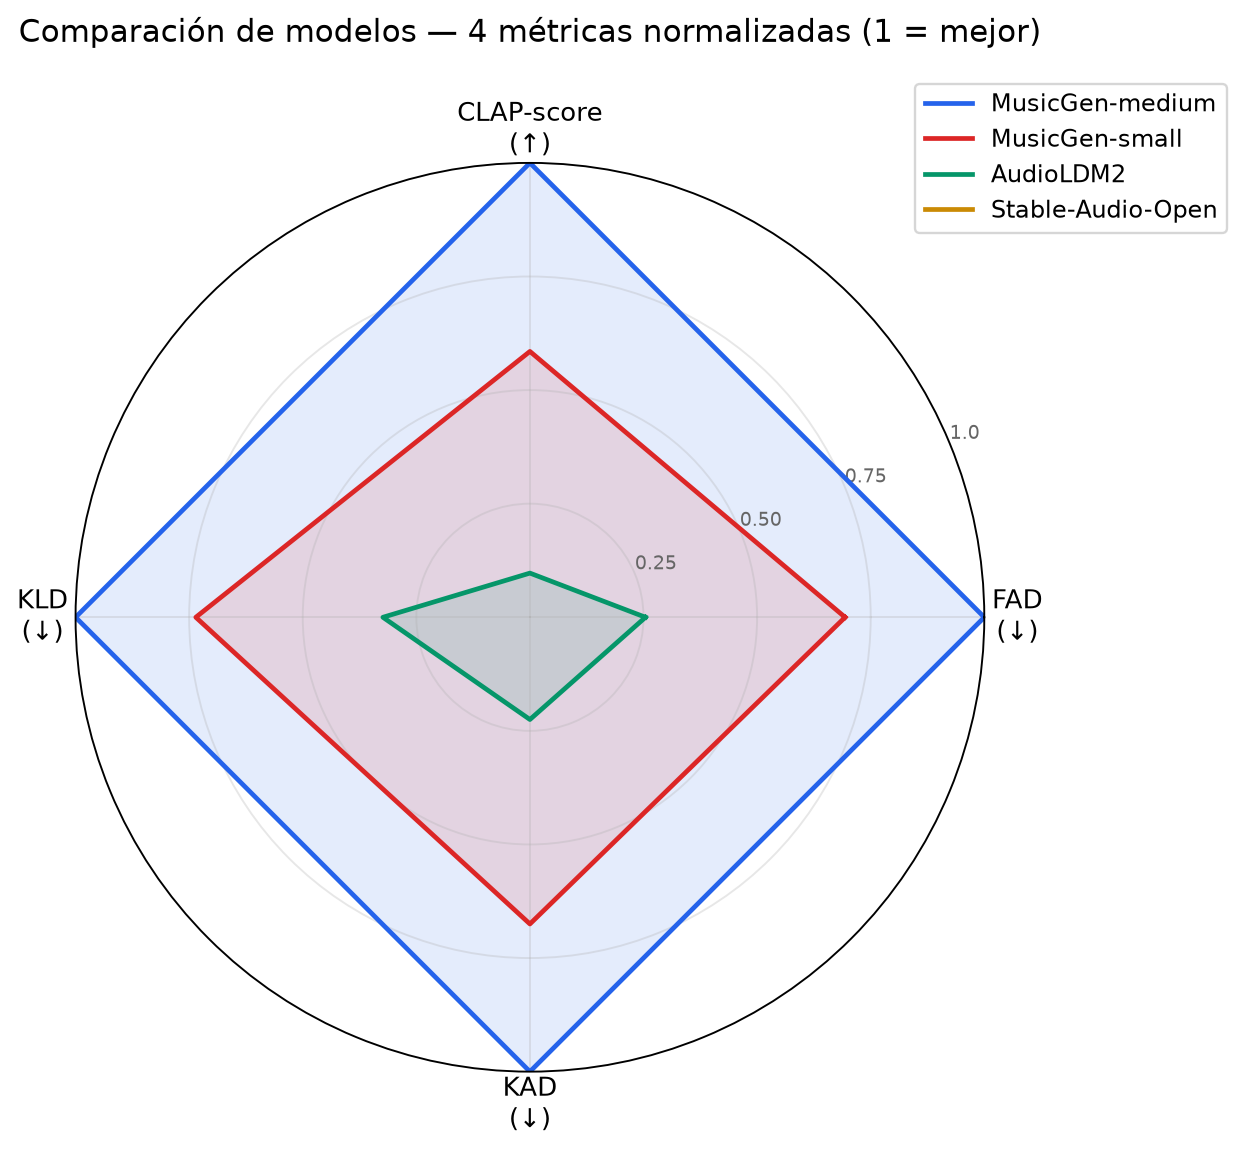
\includegraphics[width=0.85\columnwidth]{results/radar_models.png}
  \caption{Radar de comparación de modelos con las cuatro métricas
           normalizadas a $[0,\,1]$ ($1 =$ mejor).
           MusicGen-medium (azul) domina en los cuatro ejes;
           Stable-Audio-Open (amarillo) ocupa el área más pequeña.}
  \label{fig:radar}
\end{figure}

% ----------------------------------------------------------
\subsection{Discusión}
\label{sec:benchmark:discusion}

Los resultados confirman que la arquitectura basada en \textit{language
modeling} de MusicGen~\cite{copet2024simple} supera a los enfoques de
difusión latente (AudioLDM2~\cite{liu2024audioldm} y
Stable Audio Open~\cite{evans2024stable}) en todas las métricas evaluadas
sobre MusicCaps.
El análisis estadístico refuerza esta conclusión: las diferencias son
significativas a nivel omnibus ($p \approx 1.59 \times 10^{-30}$); sin
embargo, el par AudioLDM2 -- Stable-Audio-Open no alcanza significancia
estadística ($p_{\text{Bonf}} = 1.0$), lo que sugiere que ambos modelos de
difusión rinden de forma equivalente sobre el banco de 100 prompts evaluado.
Las diferencias entre los dos modelos de MusicGen sí son significativas
($p_{\text{Bonf}} = 1.6 \times 10^{-4}$) y son consistentes en los
10 géneros ($p < 0.05$ en todos).

\paragraph{Alcance: este benchmark justifica el modelo base, no la edición.}
Es importante delimitar qué evidencia aporta esta comparativa. Mide
\emph{generación texto-audio libre} sobre MusicCaps y, por tanto, sólo
respalda la \textbf{elección del modelo base} (la familia MusicGen frente a
los modelos de difusión). \textbf{No} constituye evidencia de capacidad de
\emph{edición por instrucciones}: un CLAP-score alto en generación libre no
implica preservar la identidad, la instrumentación, la estructura ni la mezcla
de una pista \emph{fuente} al aplicar una operación pedida. La tarea final del
sistema exige justamente eso. Por ello, la validación de la edición se trata
de forma separada en la Sección~\ref{sec:edit}, con un protocolo de ternas
\{fuente, instrucción, objetivo\} y líneas base específicas de edición; los
resultados de generación de esta sección no deben interpretarse como prueba de
desempeño en edición.

No obstante, conviene señalar dos limitaciones adicionales de la comparativa de
generación.
Primero, el banco de 100 prompts, aunque balanceado por género, no cubre la
larga cola de estilos y sub-géneros presentes en aplicaciones reales.
Segundo, las métricas automáticas capturan fidelidad distribucional y
coherencia semántica texto-audio, pero no sustituyen a la evaluación
subjetiva de calidad musical percibida.
Ambas limitaciones se abordarán en trabajo futuro mediante la ampliación del
banco de pruebas y la incorporación de una evaluación de escucha controlada
(\textit{MUSHRA}~\cite{series2014method}).

% ============================================================
%  Referencias sugeridas (agregar al .bib principal)
% ============================================================
%
% @inproceedings{agostinelli2023musiclm,
%   title={{MusicLM}: Generating Music From Text},
%   author={Agostinelli, Andrea and others},
%   booktitle={arXiv preprint arXiv:2301.11325}, year={2023}}
%
% @inproceedings{kilgour2019fad,
%   title={Fr\'echet Audio Distance: A Reference-Free Metric for Evaluating Music Enhancement Algorithms},
%   author={Kilgour, Kevin and others},
%   booktitle={Interspeech}, year={2019}}
%
% @inproceedings{wu2023large,
%   title={{CLAP}: Learning Audio Concepts From Natural Language Supervision},
%   author={Wu, Yusong and others},
%   booktitle={ICASSP}, year={2023}}
%
% @inproceedings{copet2024simple,
%   title={Simple and Controllable Music Generation},
%   author={Copet, Jade and others},
%   booktitle={NeurIPS}, year={2024}}
%
% @inproceedings{liu2024audioldm,
%   title={{AudioLDM} 2: Learning Holistic Audio Generation With Self-Supervised Pretraining},
%   author={Liu, Haohe and others},
%   booktitle={TASLP}, year={2024}}
%
% @inproceedings{evans2024stable,
%   title={Stable Audio Open},
%   author={Evans, Zach and others},
%   booktitle={arXiv preprint arXiv:2407.14358}, year={2024}}
%
% @inproceedings{huang2023make,
%   title={Make-An-Audio: Text-To-Audio Generation With Prompt-Enhanced Diffusion Models},
%   author={Huang, Rongjie and others},
%   booktitle={ICML}, year={2023}}
%
% @article{kruskal1952use,
%   title={Use of Ranks in One-Criterion Variance Analysis},
%   author={Kruskal, William H. and Wallis, W. Allen},
%   journal={JASA}, volume={47}, number={260}, pages={583--621}, year={1952}}
%
% @article{dunn1964multiple,
%   title={Multiple Comparisons Using Rank Sums},
%   author={Dunn, Olive Jean},
%   journal={Technometrics}, volume={6}, number={3}, pages={241--252}, year={1964}}
%
% @techreport{series2014method,
%   title={Method for the Subjective Assessment of Intermediate Quality Level of Audio Systems},
%   author={{ITU-R}},
%   institution={ITU}, number={BS.1534-3}, year={2014}}
